\section{Qgis}
\begin{frame}
    \begin{figure}
        \centering
        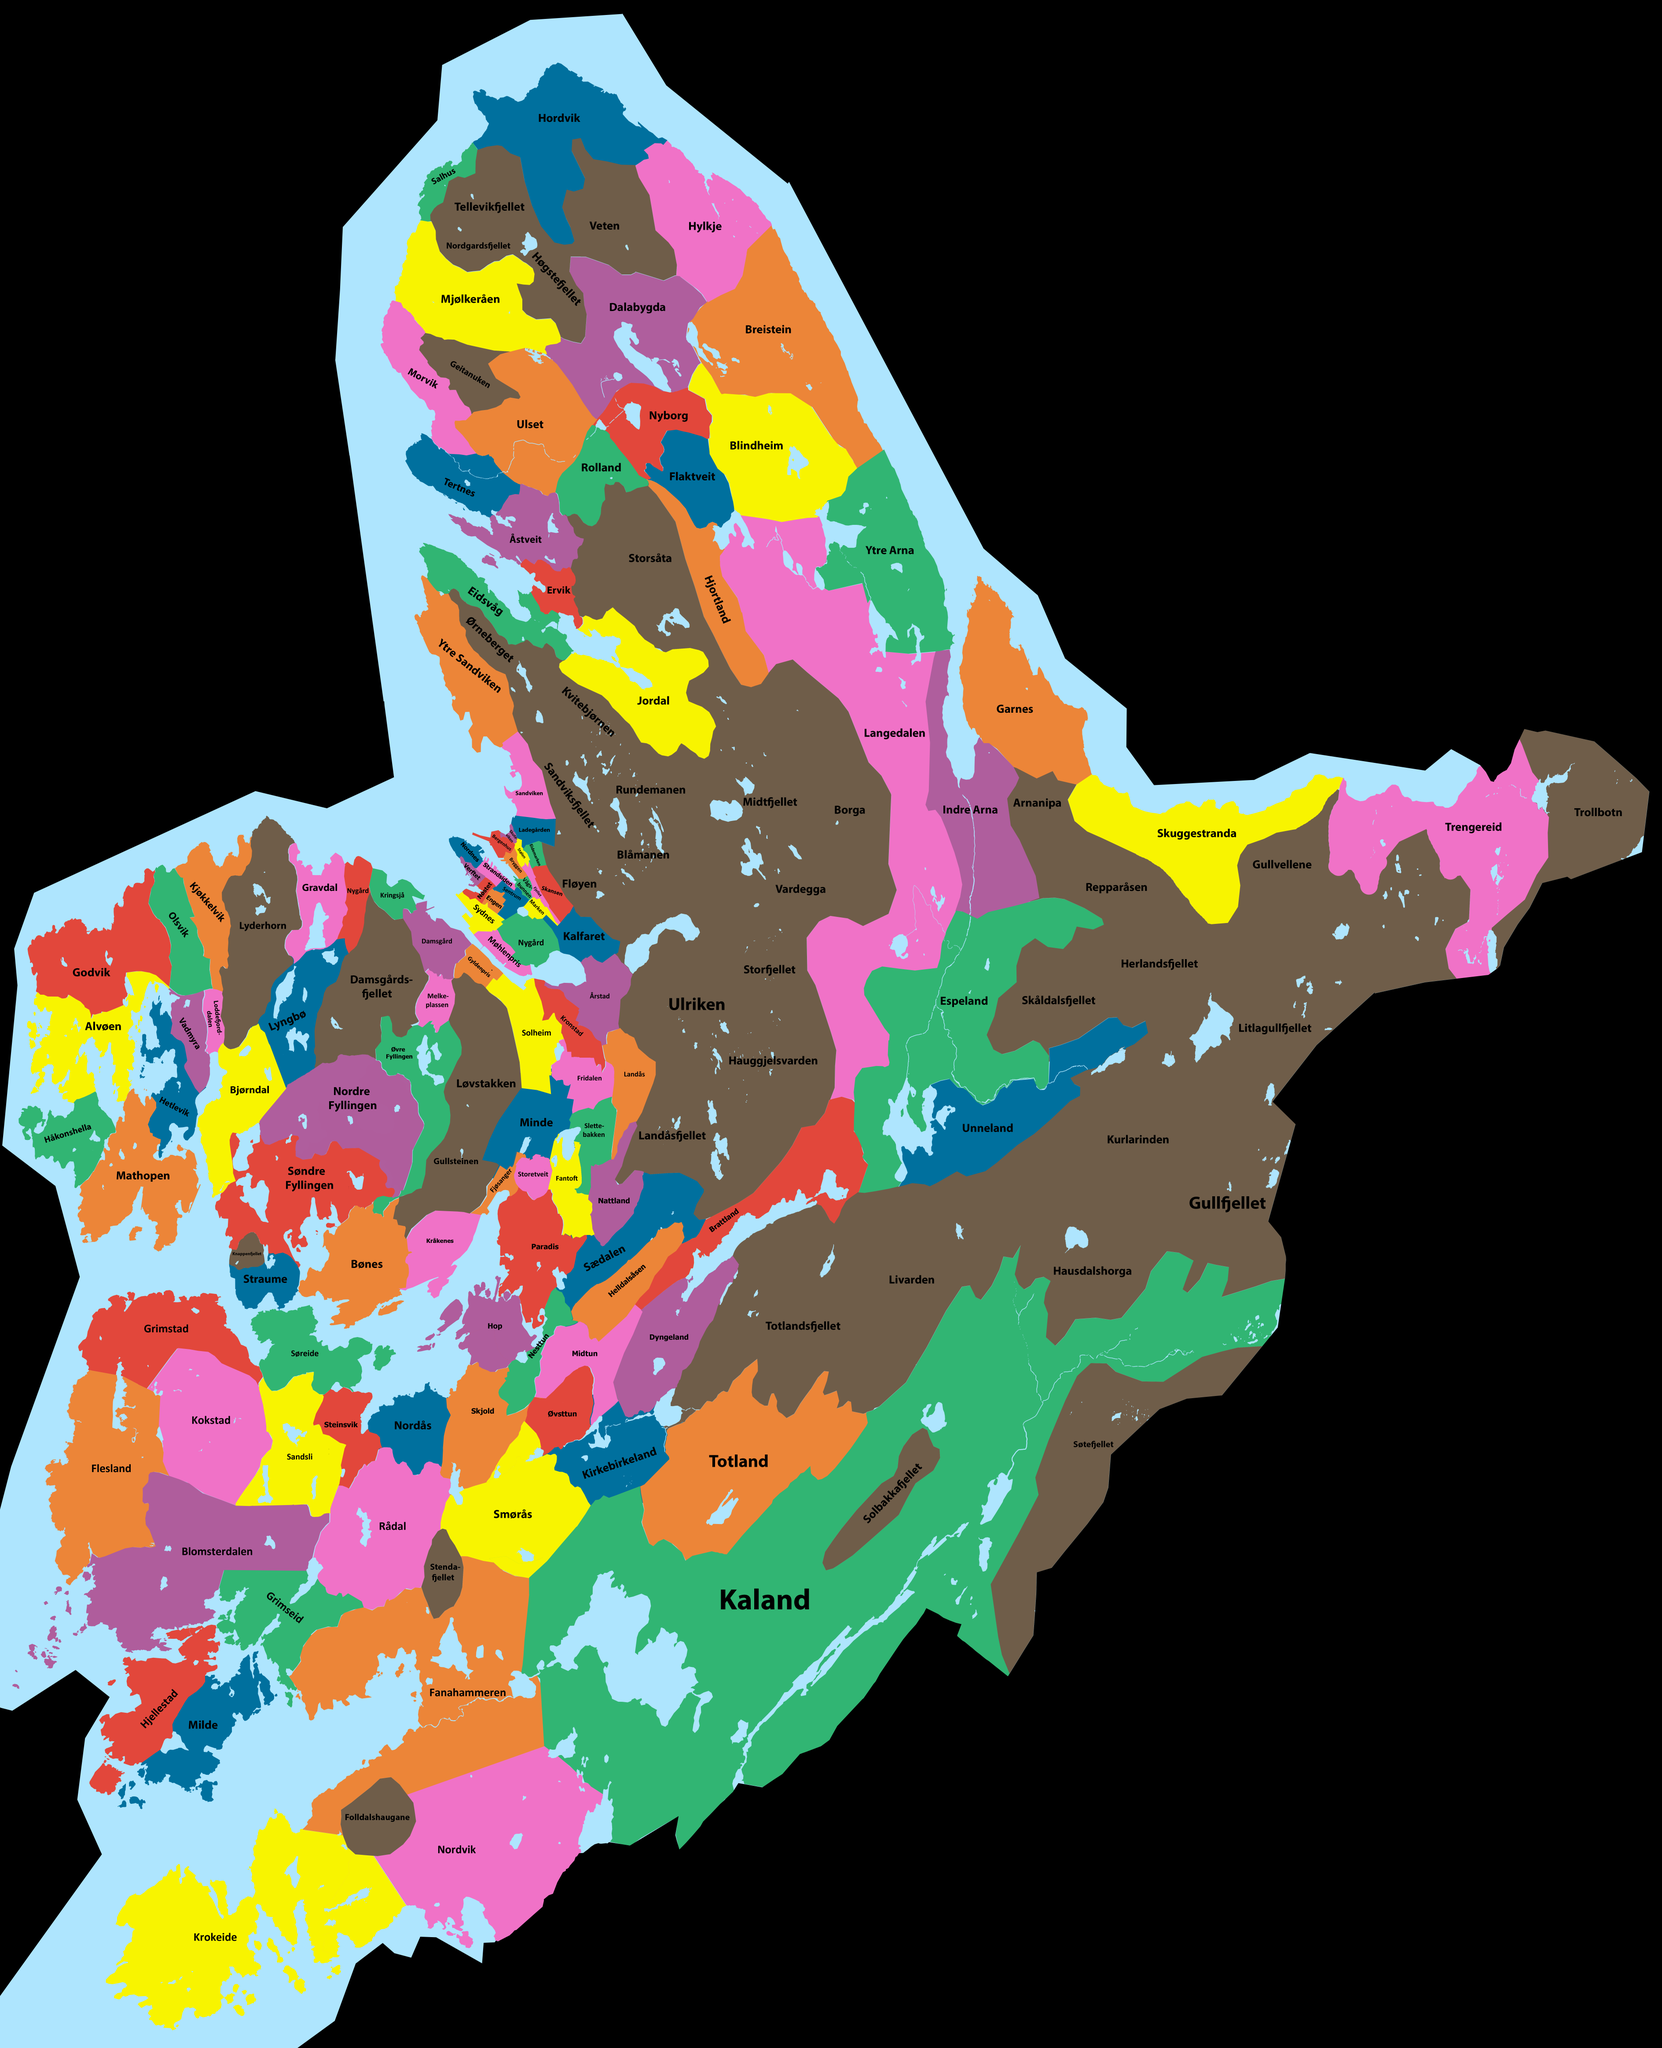
\includegraphics[height = 6cm]{images/boligomraaderWiki.png}%
        \caption{Geography of Bergen - The truth}
    \end{figure}
\end{frame}

\begin{frame}
    \begin{itemize}[<+->]
        \item Original is a PNG file, not SVG
        \item $\Rightarrow$ Contact author about data source
        \item $\Rightarrow$ No answer
        \item Try to unassemble by using different tools (AI sucks)
        \item $\Rightarrow$ No success
    \end{itemize}
\end{frame}

\begin{frame}
    \begin{figure}
        \centering
        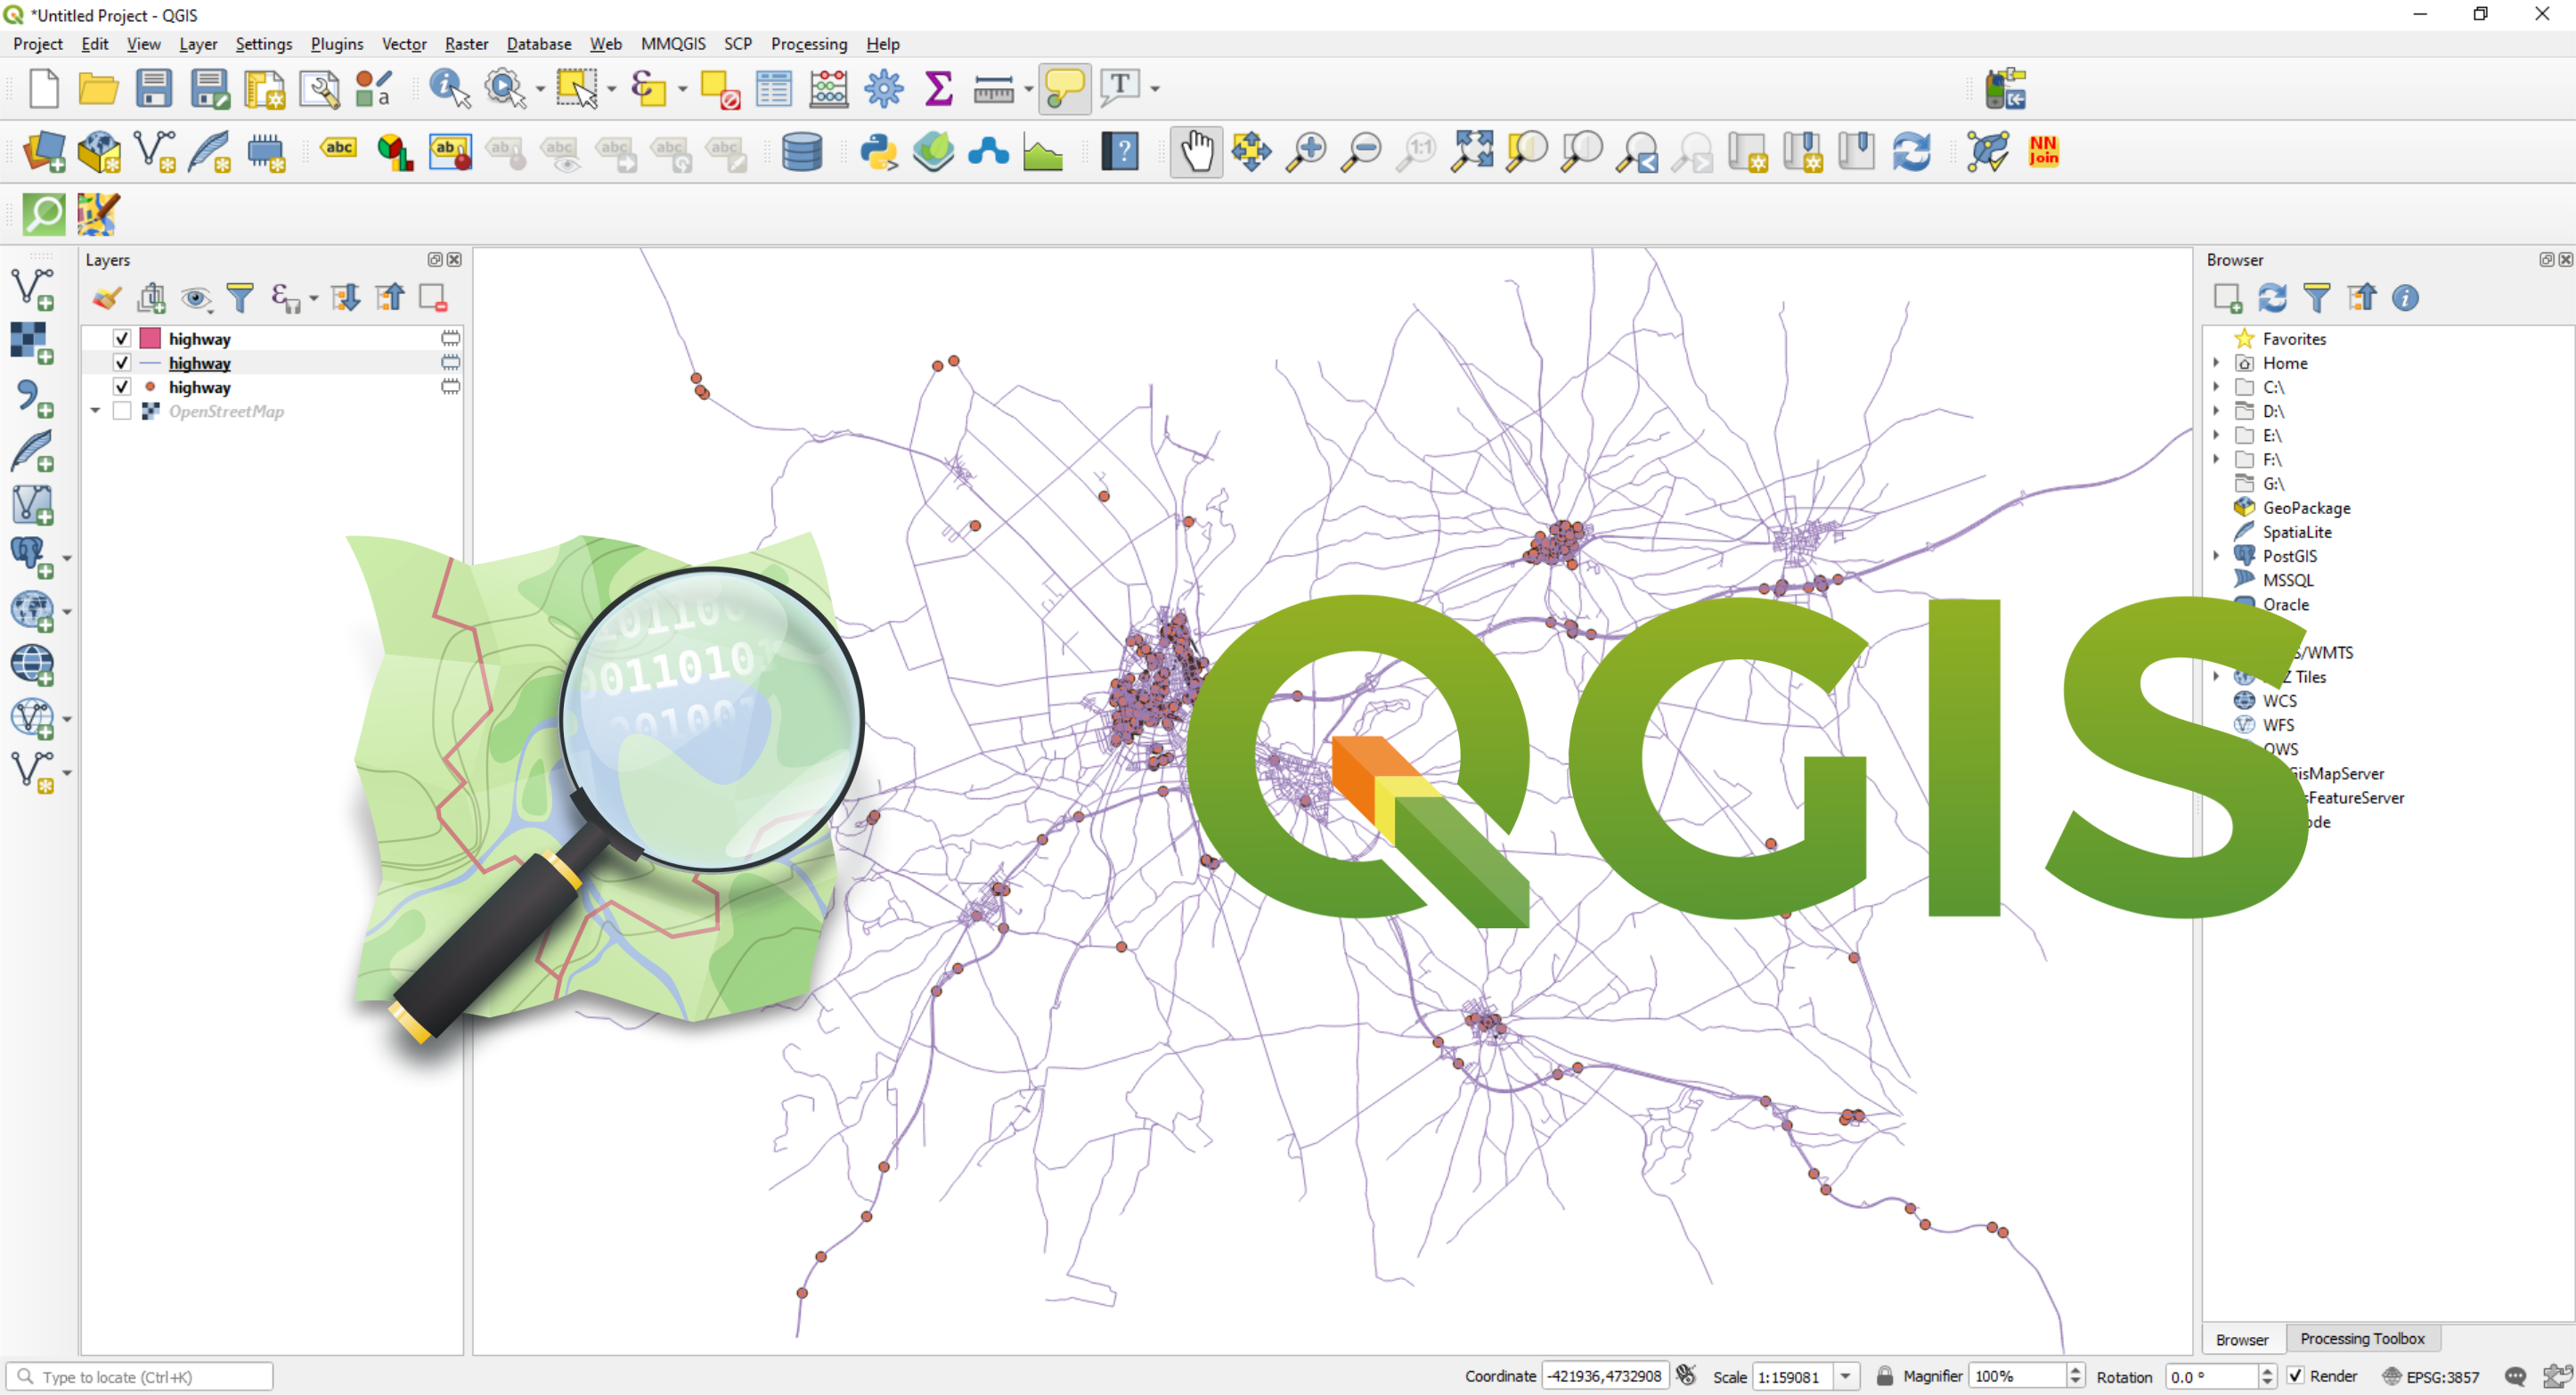
\includegraphics[height = 6cm]{images/qgis.png}%
        \caption{Qgis - A programme of horror}
    \end{figure}
\end{frame}

\begin{frame}{Settings}
    \begin{itemize}[<+->]
        \item Click through six pages of settings to set up a project
        \item Let's learn 5 years of cartography studies in one hour
        \item Projection? Mercator?
        \pause
        \begin{block}{Stackoverflow}
            \enquote{Of course you have to use the EPSG:25832 projection for the type of project you are working with.}
        \end{block}
    \end{itemize}
\end{frame}

\begin{frame}
    \begin{figure}
        \centering
        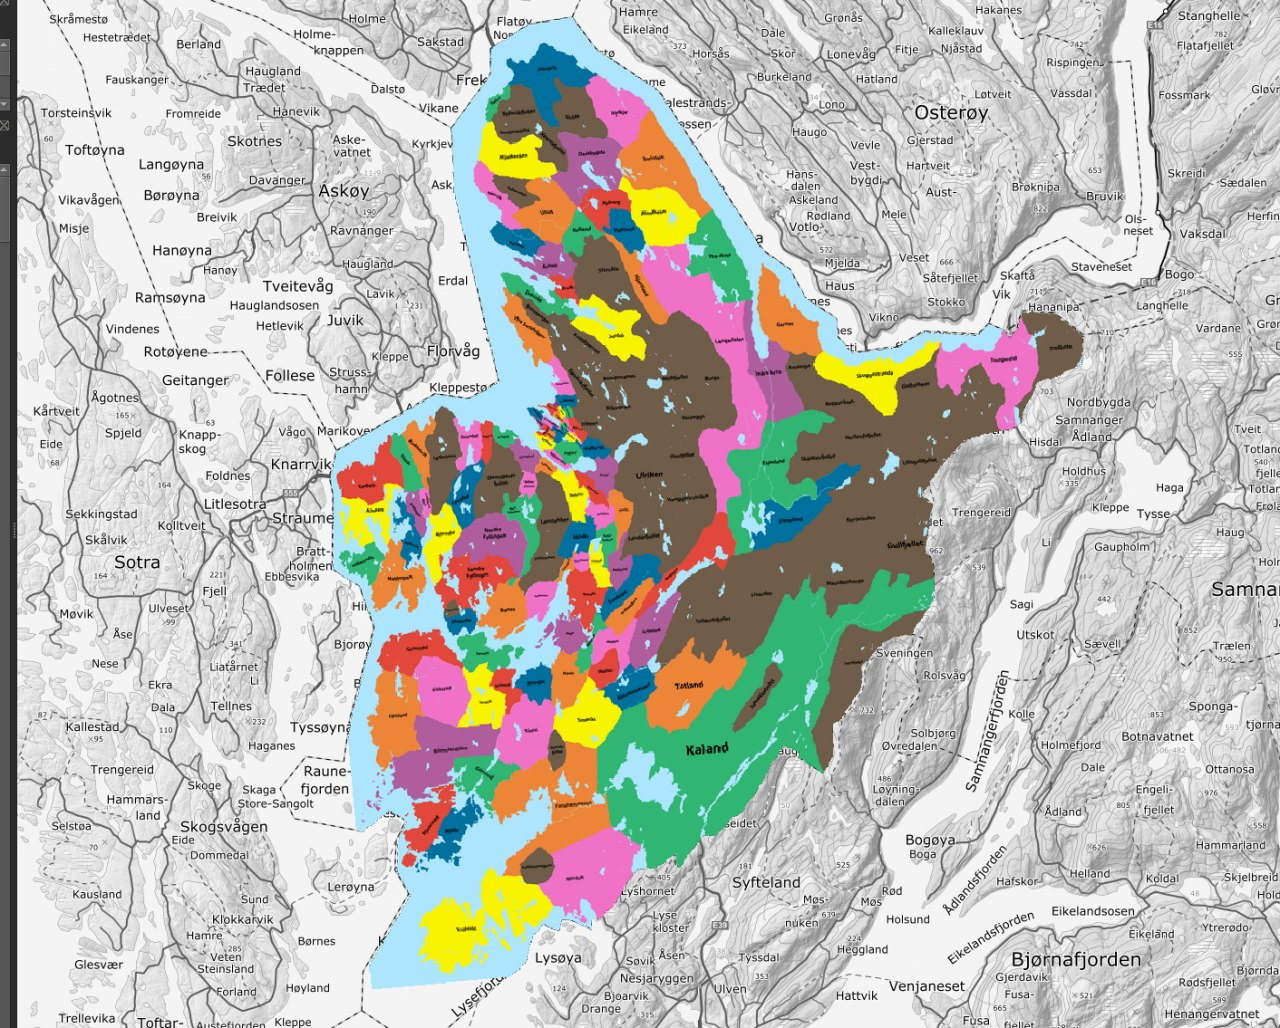
\includegraphics[height = 6cm]{images/qgis1.jpg}%
        \caption{Initialise correct layers}
    \end{figure}
\end{frame}

\begin{frame}
    \begin{figure}
        \centering
        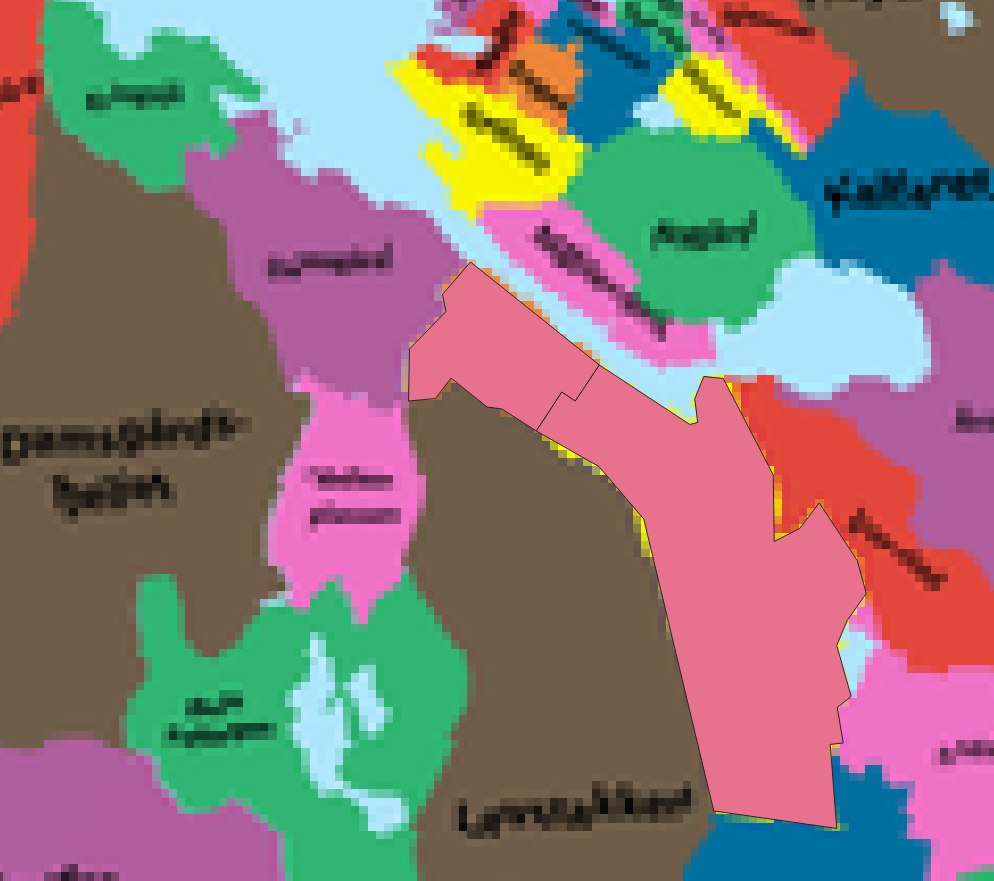
\includegraphics[height = 6cm]{images/qgis2.png}%
        \caption{Draw some borders}
    \end{figure}
\end{frame}

\begin{frame}
    \begin{figure}
        \centering
        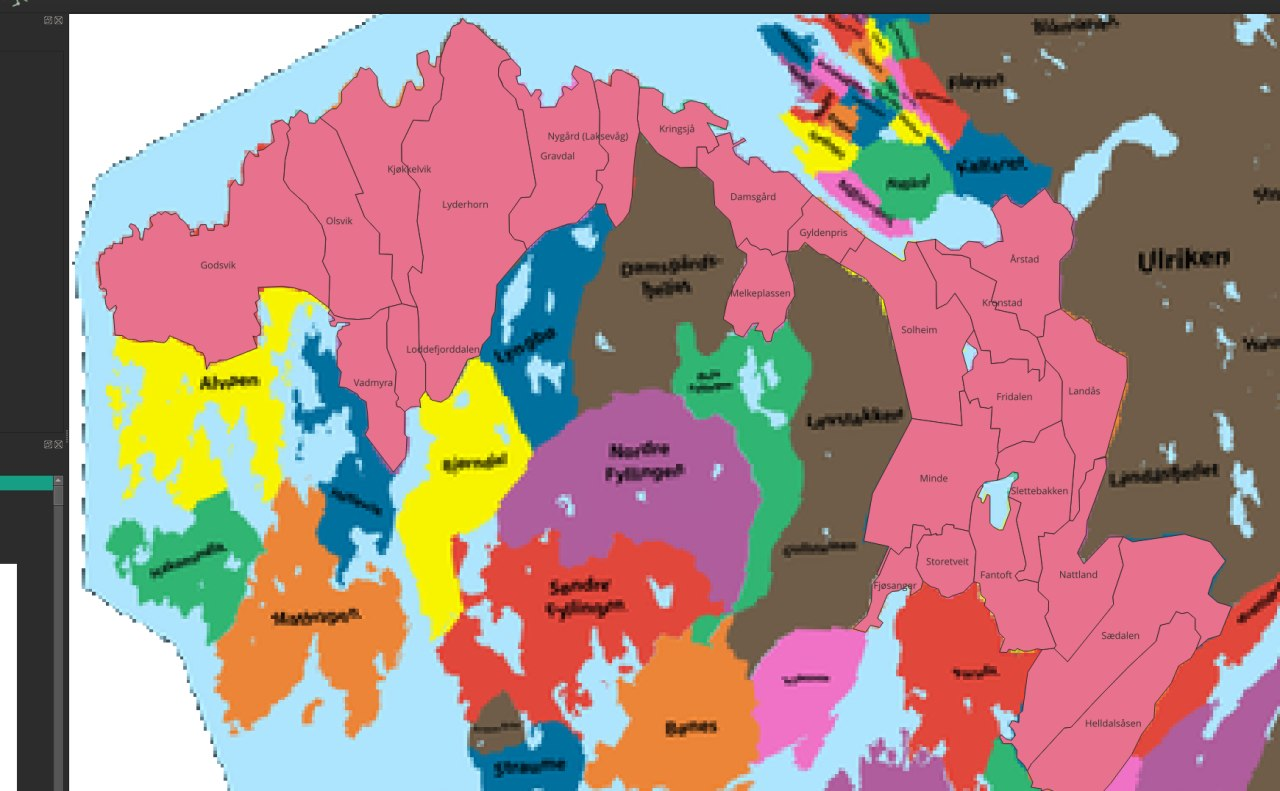
\includegraphics[height = 6cm]{images/qgis3.jpg}%
        \caption{More drawing}
    \end{figure}
\end{frame}

\begin{frame}
    \begin{figure}
        \centering
        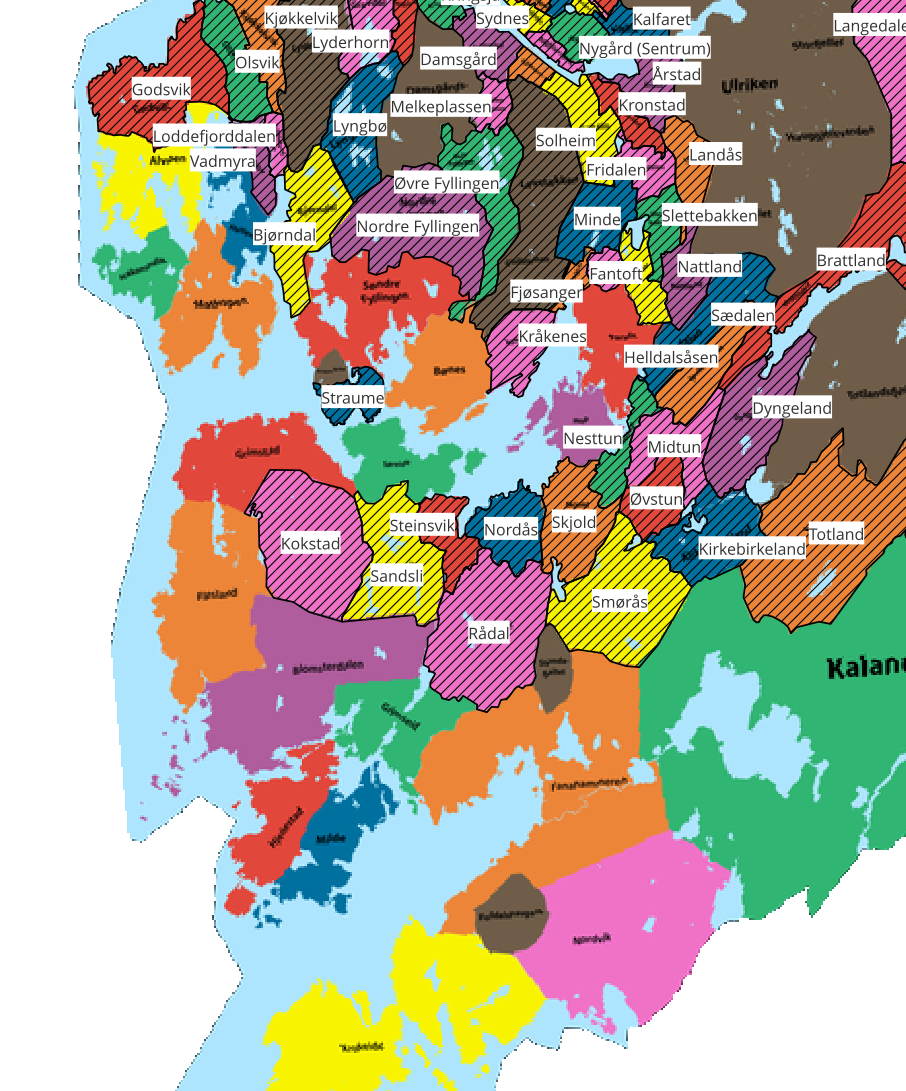
\includegraphics[height = 6cm]{images/qgis4.png}%
        \caption{Even more drawing}
    \end{figure}
\end{frame}

%\begin{frame}
%    \begin{figure}
%        \centering
%        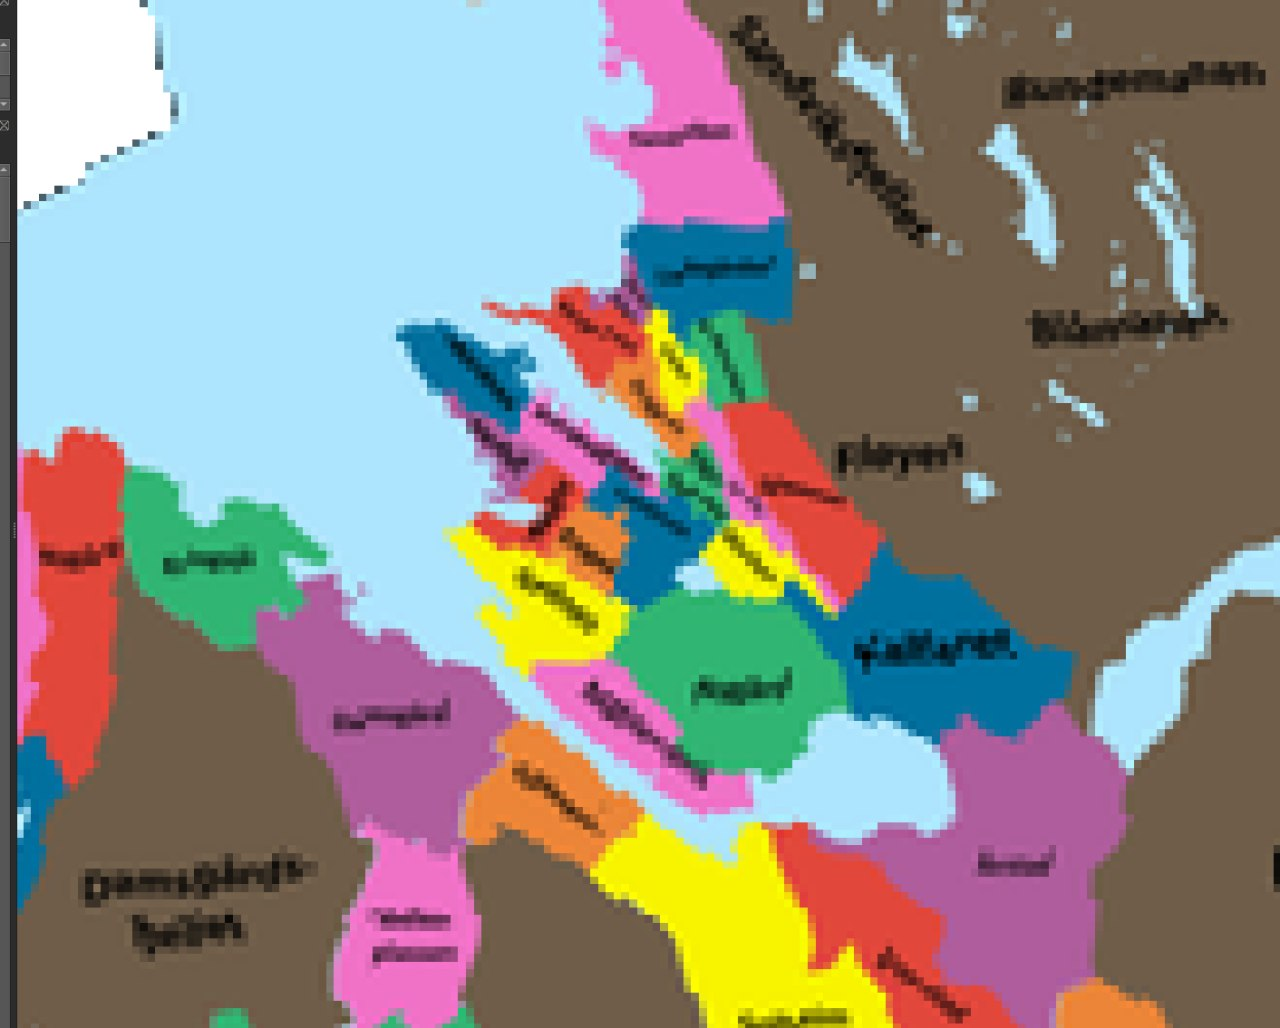
\includegraphics[height = 6cm]{images/qgis5.png}%
%        \caption{Sentrum???}
%    \end{figure}
%\end{frame}

\begin{frame}
    \begin{figure}
        \centering
        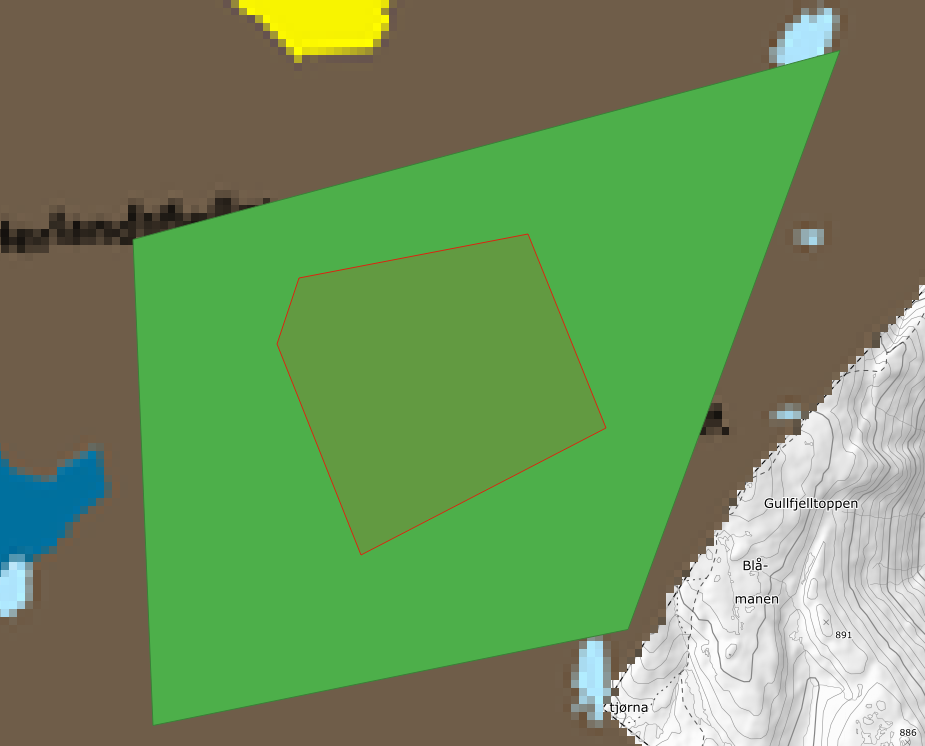
\includegraphics[height = 6cm]{images/qgis_shapeInShape.png}%
        \caption{Lakes? \enquote{The inserted ring is not contained in the other ring.}}
    \end{figure}
\end{frame}

%\begin{frame}
%   \begin{figure}
%        \centering
%        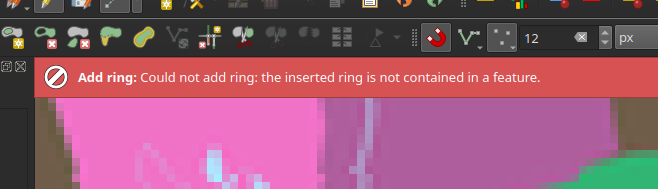
\includegraphics[height = 4cm]{images/qgis_ringInRing.png}%
%        \caption{Er EPSG:25832 det man ser?}
%    \end{figure}
%\end{frame}

\begin{frame}
    \begin{figure}
        \centering
        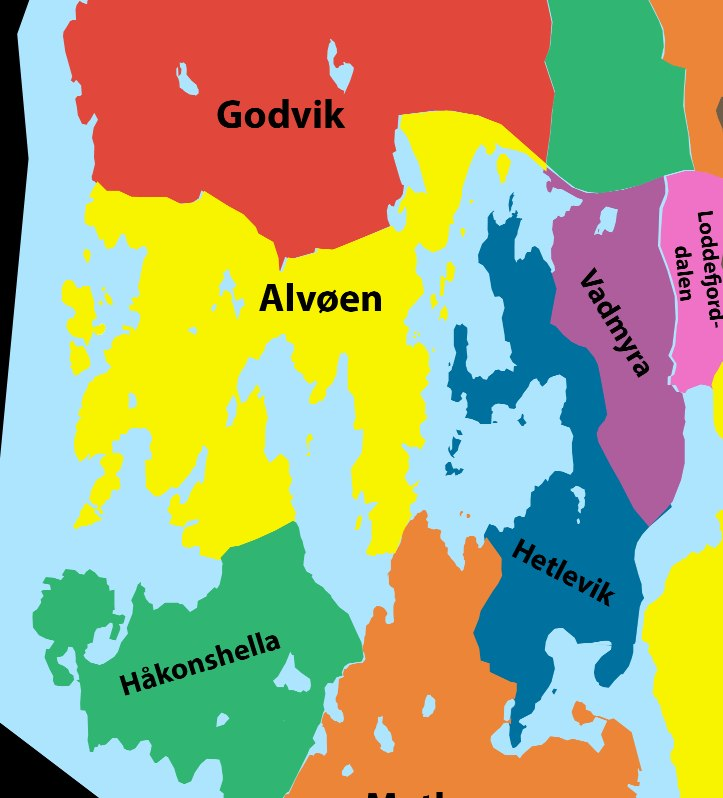
\includegraphics[height = 6cm]{images/qgis_islands.jpg}%
        \caption{Islands? \enquote{Could not add multi part element. This layer (type multilayer) does not support multi layer elements.}}
    \end{figure}
\end{frame}

\begin{frame}
    \begin{figure}
        \centering
        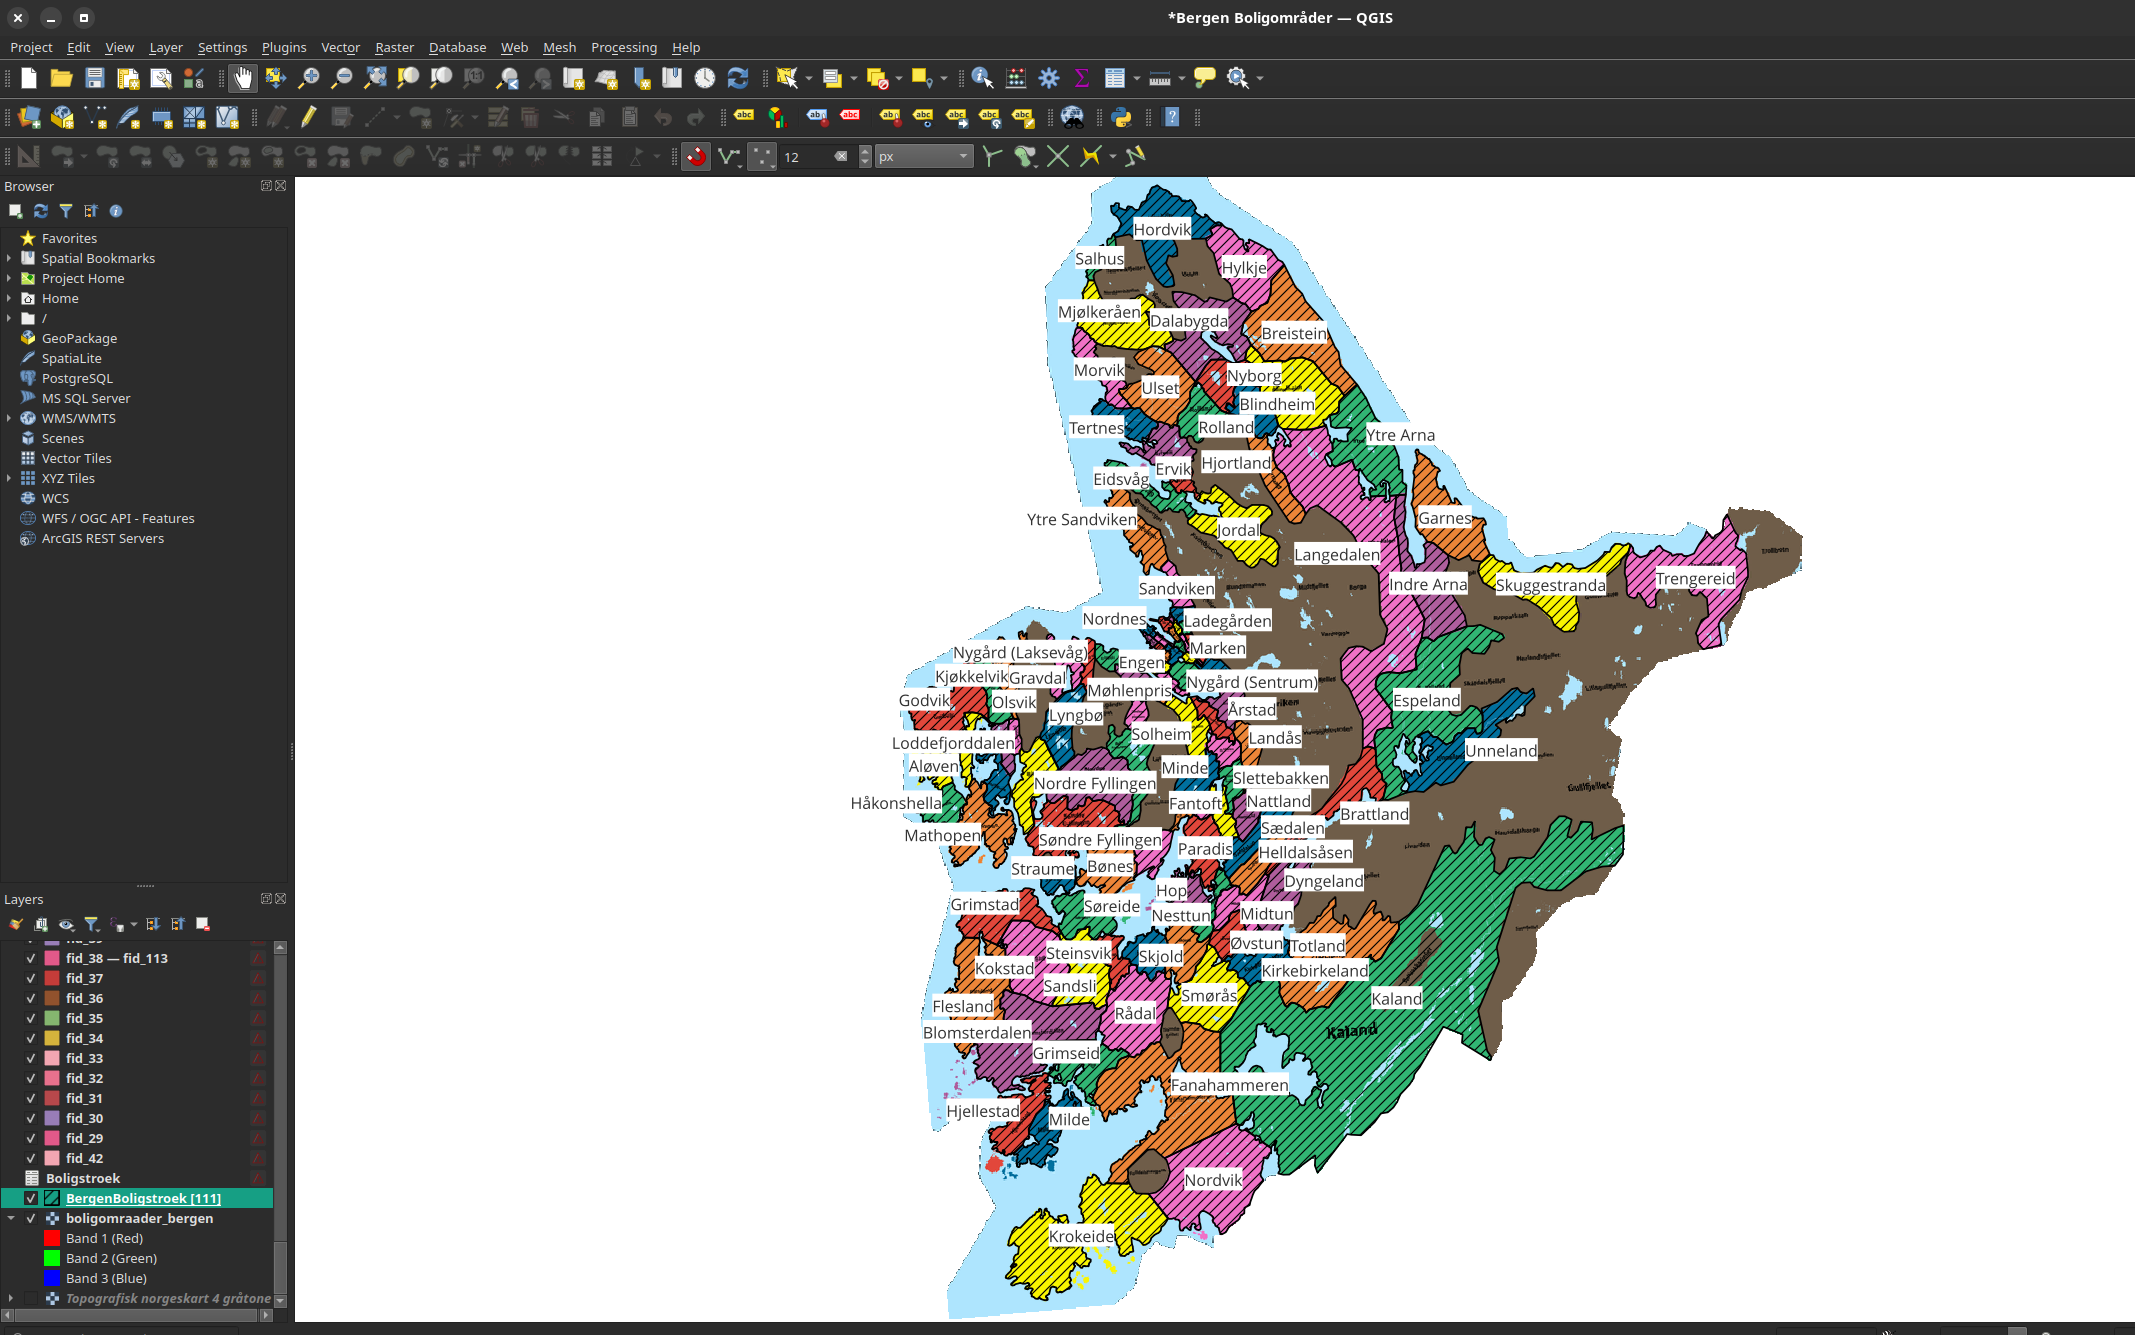
\includegraphics[height = 6cm]{images/qgisOverview.png}%
        \caption{Finally}
    \end{figure}
\end{frame}

%\begin{frame}
%    \begin{alertblock}{Error}
%        \enquote{Could not add multi part element. This layer (type multilayer) does not support multi layer elements.}
%    \end{alertblock}
%    \begin{figure}
%        \centering
%        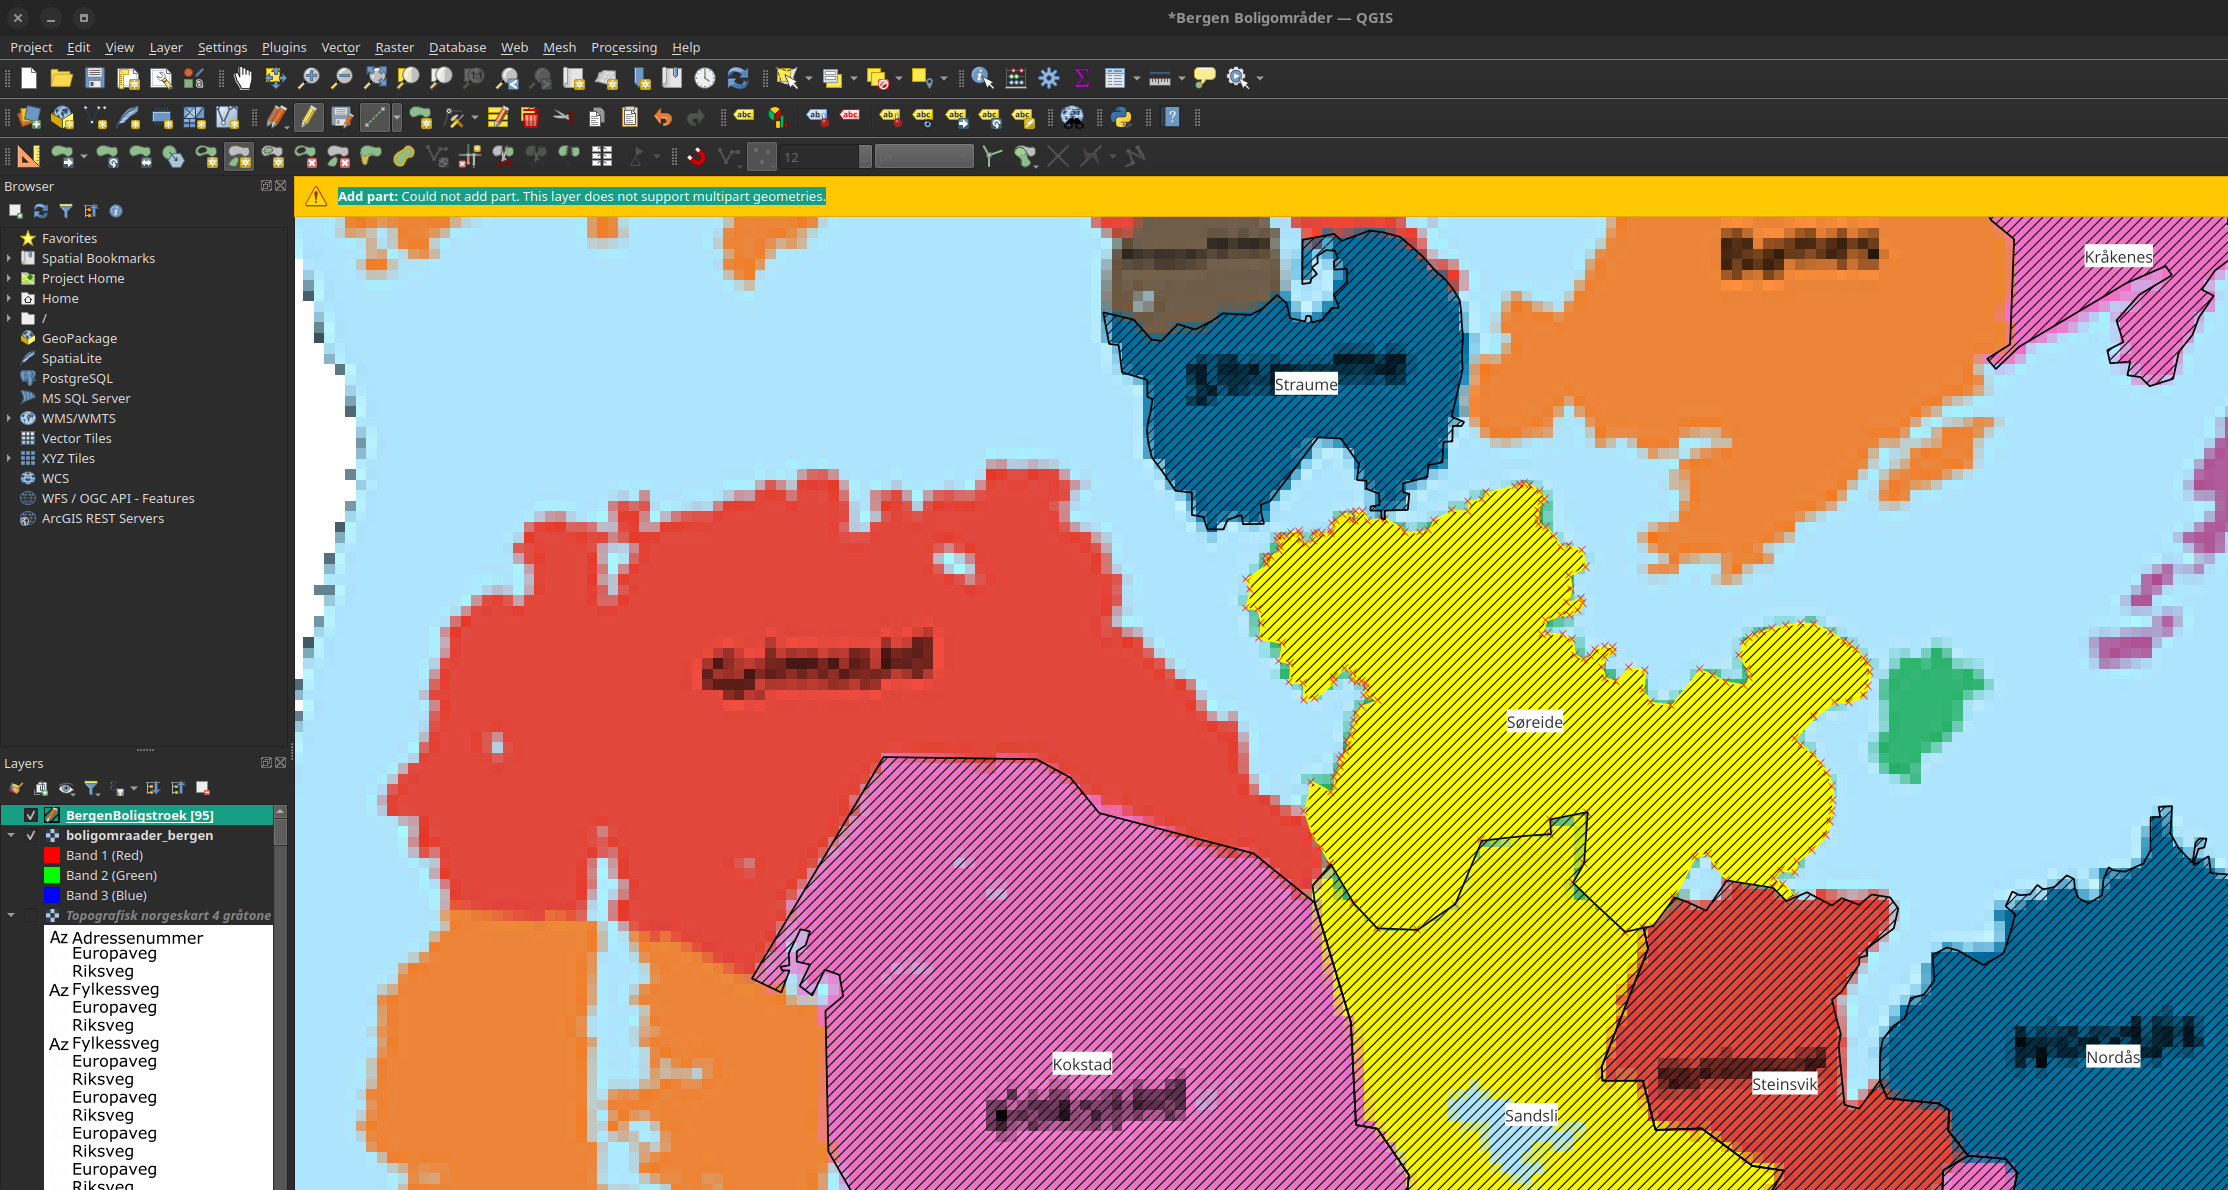
\includegraphics[height = 6cm]{images/qgis_multipart.png}%
%        \caption{}
%    \end{figure}
%\end{frame}

% ====================================
\subsection{Export}
\begin{frame}
    \begin{figure}
        \centering
        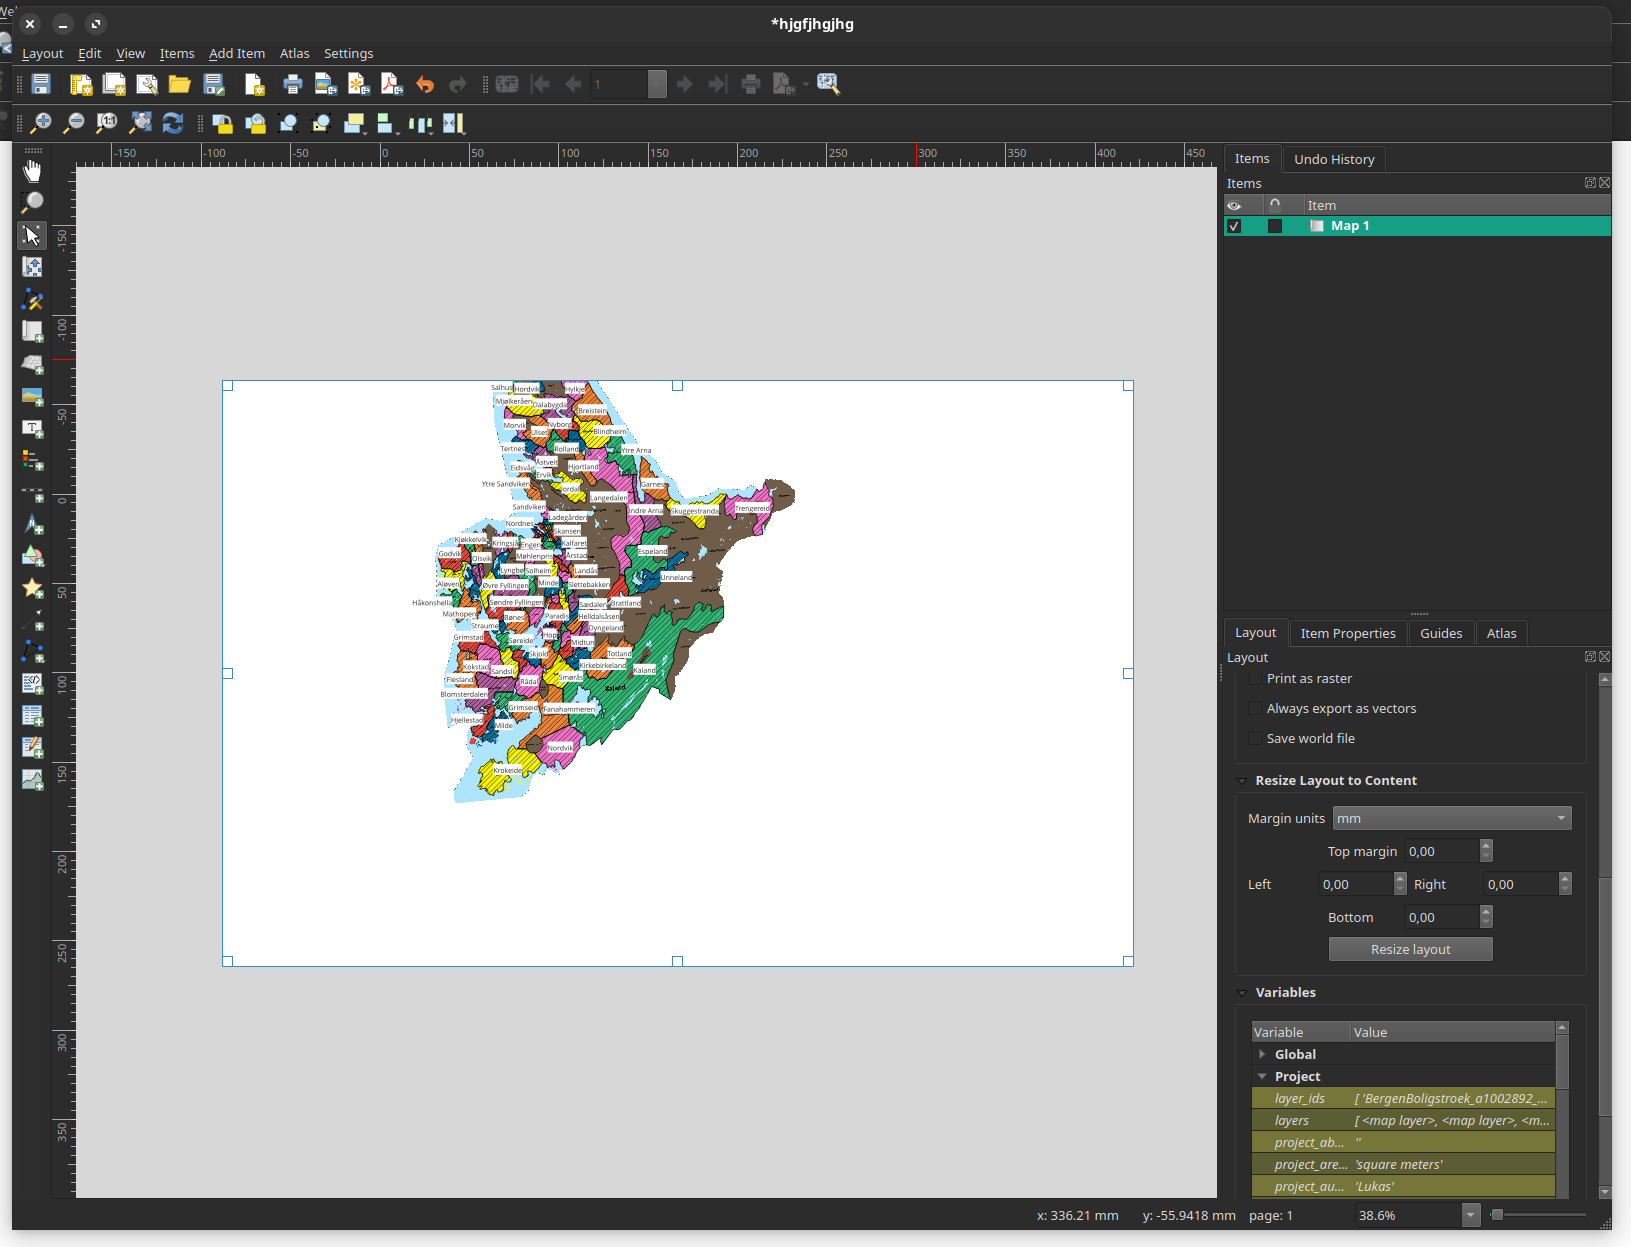
\includegraphics[height = 6cm]{images/qgis_export.png}%
        \caption{Ka e det?}
    \end{figure}
\end{frame}

\begin{frame}
    \begin{block}{Stackoverflow}
        \enquote{You have to select \textit{Vector Data Management Tools Split Vector Layer} on page 4 of the print menu. This will give you one SVG for the entire area and then you can dismantle the SVG file.}
    \end{block}
\end{frame}


\begin{frame}
    \begin{figure}
        \centering
        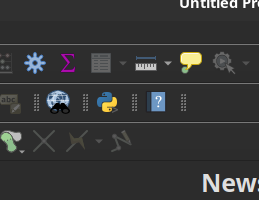
\includegraphics[height = 6cm]{images/qgis_python.png}%
        \caption{Insert Python?}
    \end{figure}
\end{frame}

\begin{frame}
    \begin{figure}
        \centering
        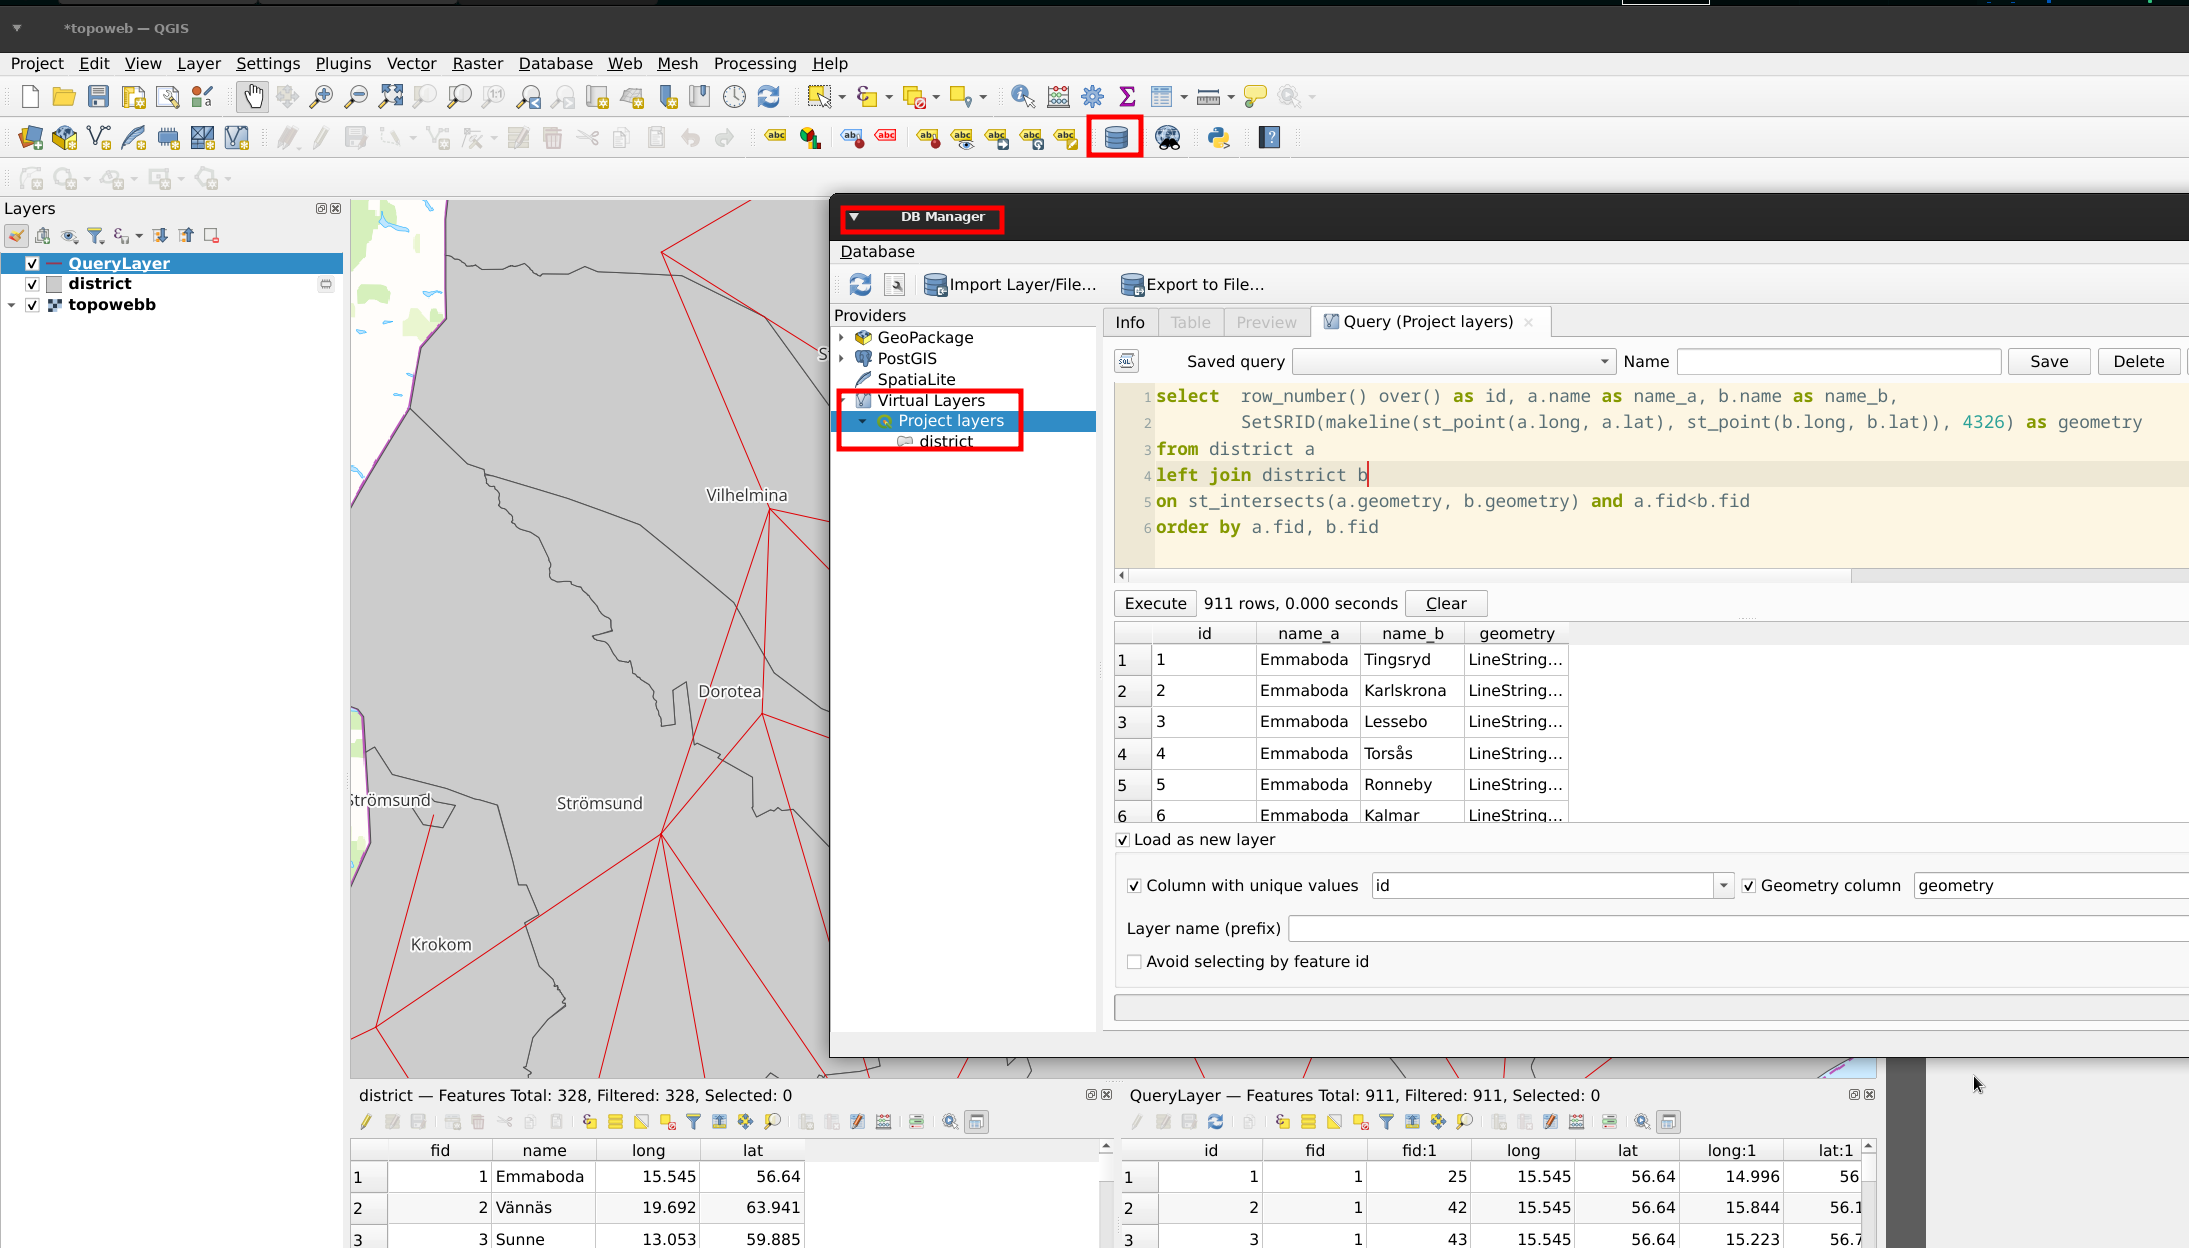
\includegraphics[height = 6cm]{images/qgis_sql.png}%
        \caption{Inline SQL}
    \end{figure}
\end{frame}

\begin{frame}
    \begin{figure}
        \centering
        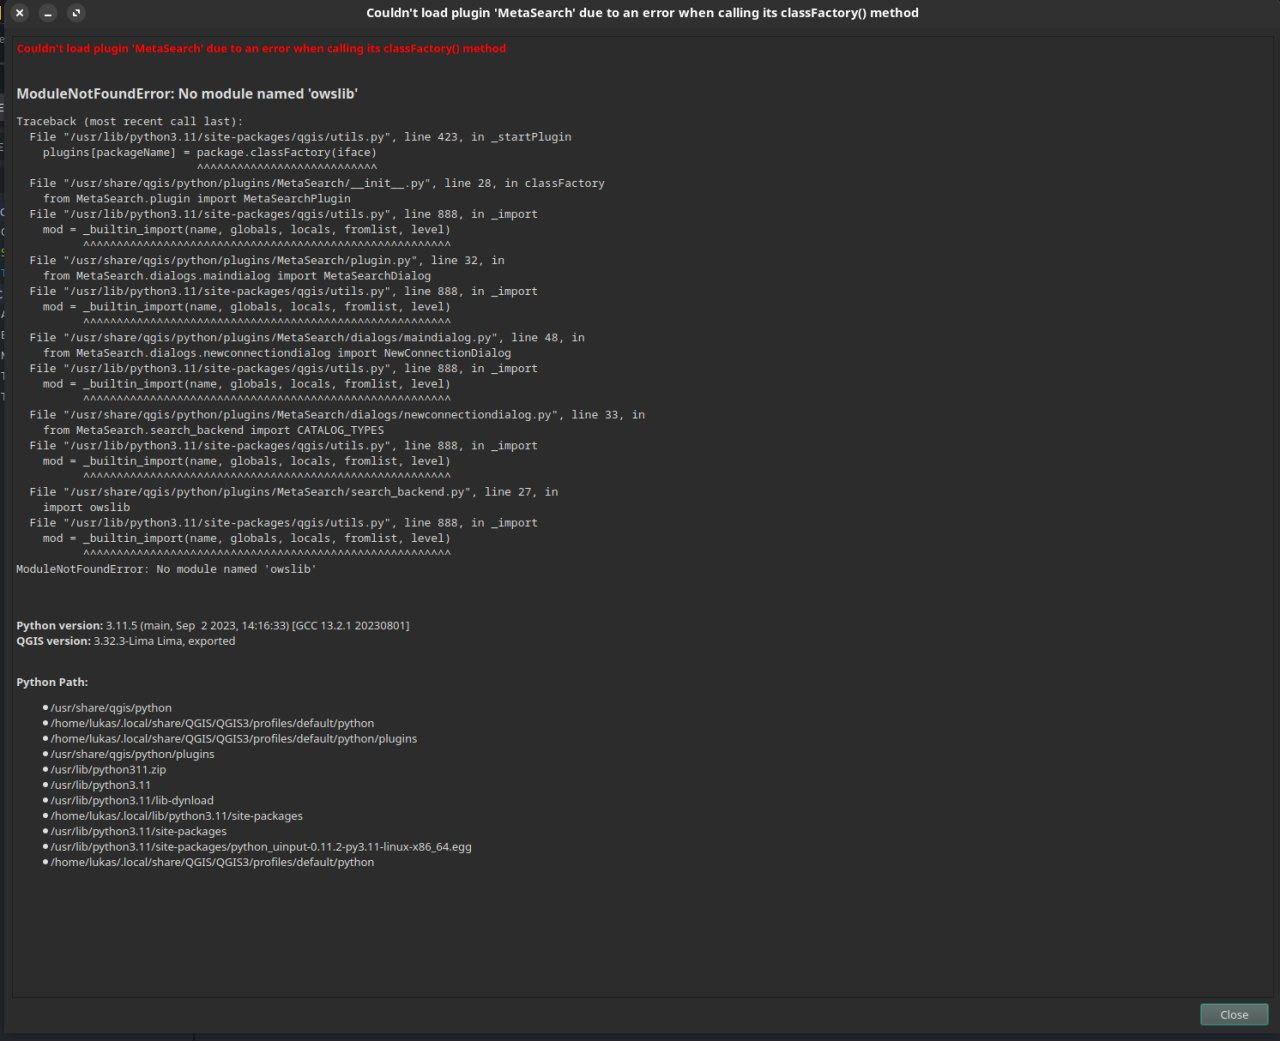
\includegraphics[height = 6cm]{images/qgis_pythonerror.jpg}%
        \caption{Python-Error}
    \end{figure}
\end{frame}

\begin{frame}
    \begin{figure}
        \centering
        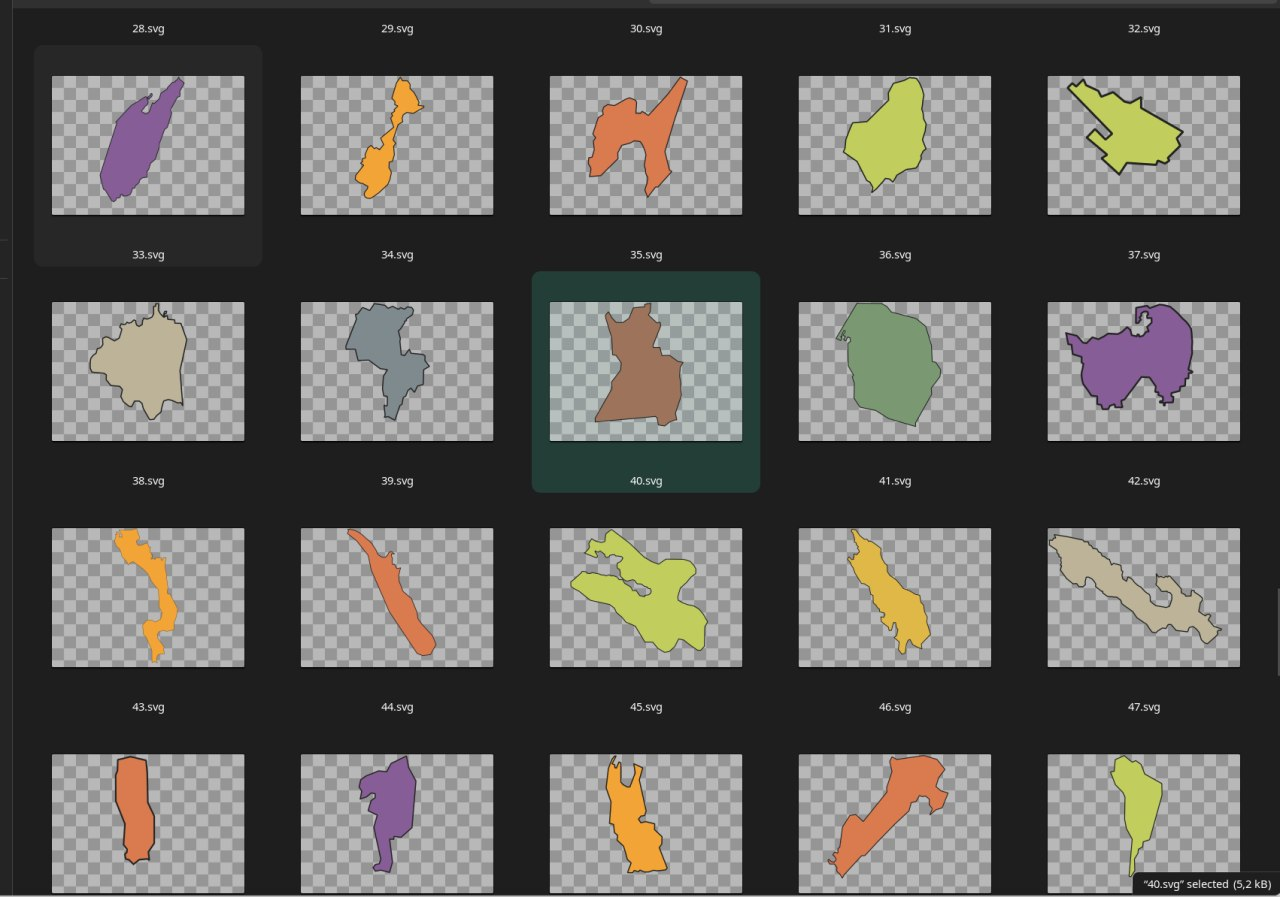
\includegraphics[height = 6cm]{images/svg_finished.jpg}%
        \caption{Finally!}
    \end{figure}
\end{frame}

\begin{frame}
    \begin{figure}
        \centering
        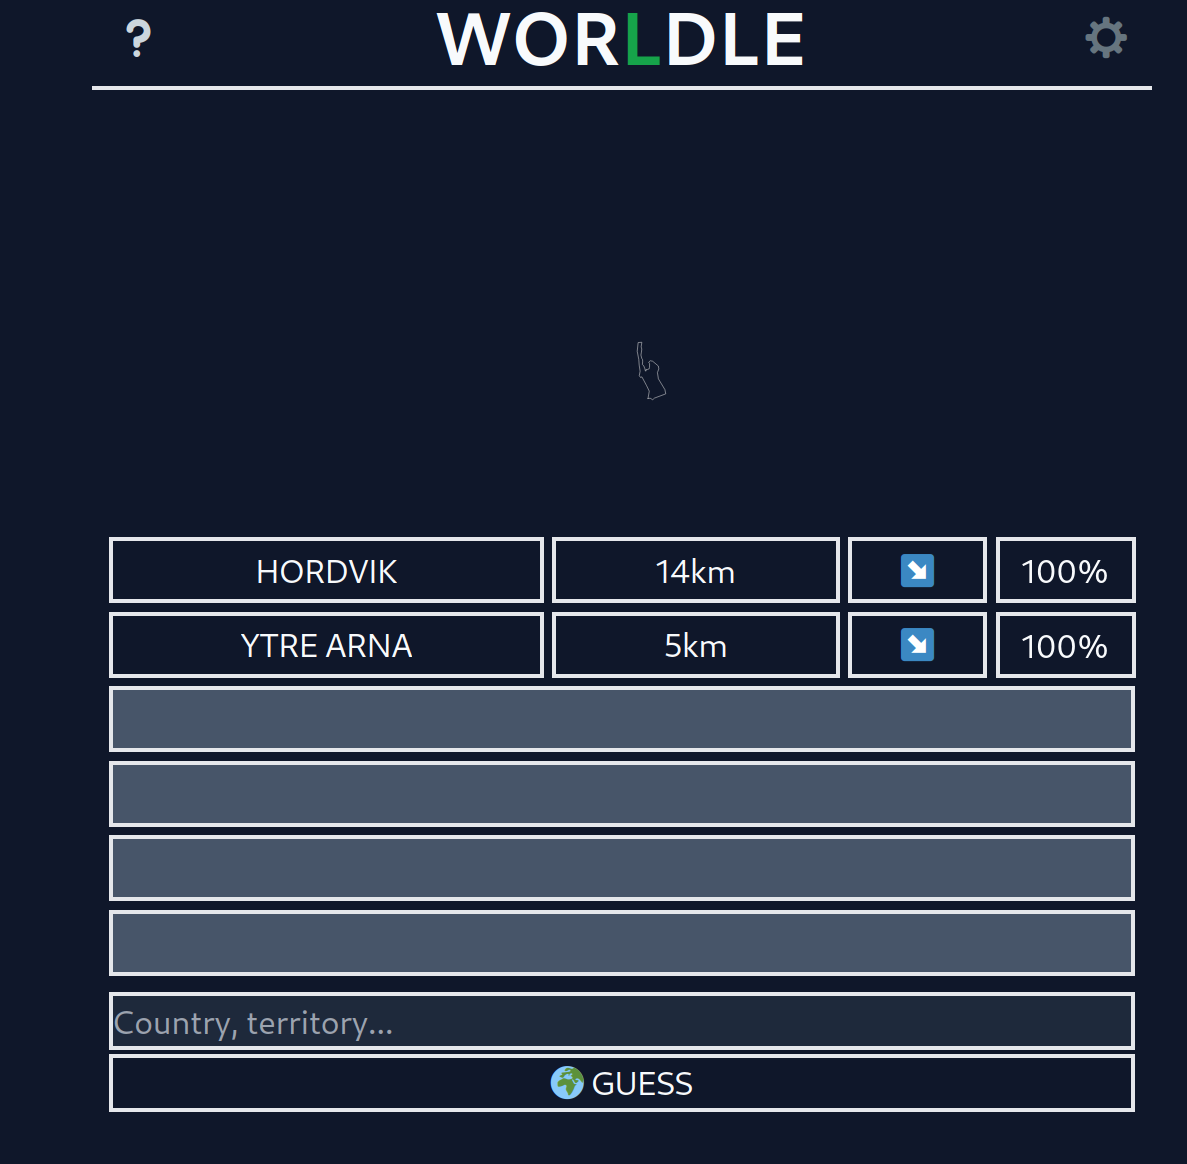
\includegraphics[height = 6cm]{images/svg_toosmall.png}%
        \caption{Wrong SVG-file sizes}
    \end{figure}
\end{frame}

\subsection{Finished website}
\begin{frame}
    \begin{figure}
        \centering
        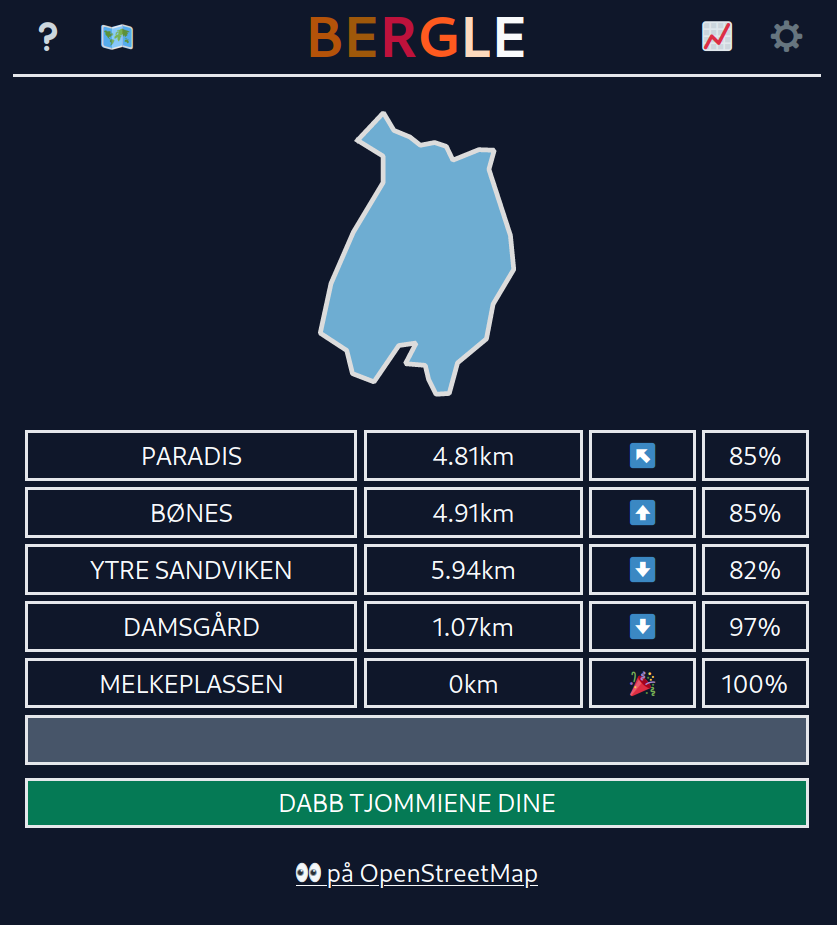
\includegraphics[height = 6cm]{images/bergleFinal.png}%
        \caption{Bergle}
    \end{figure}
\end{frame}

\subsection{Map function}
\begin{frame}
    \begin{figure}
        \centering
        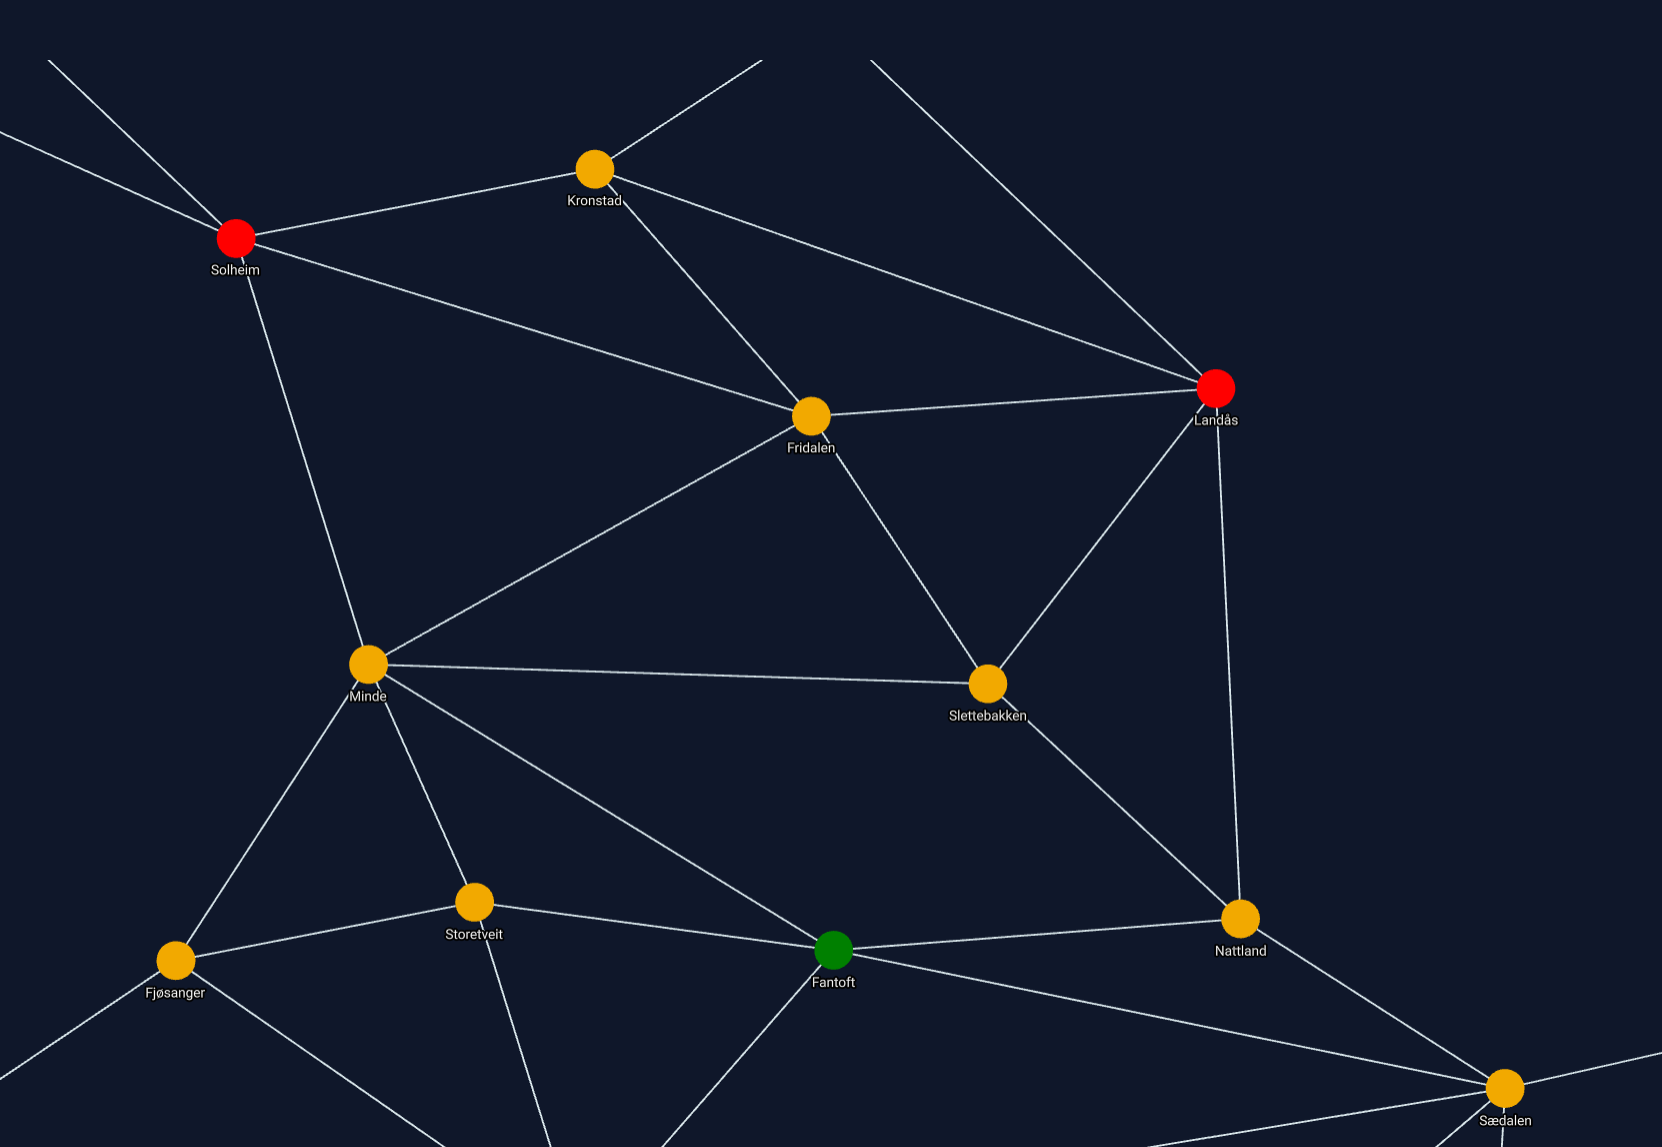
\includegraphics[height = 6cm]{images/map.png}%
        \caption{New map helper function (beta!)}
    \end{figure}
\end{frame}

\subsection{Compass function}
\begin{frame}
    \begin{columns}[t]
        \begin{column}{.4\textwidth}
        \vspace{-0.5cm}
        \hspace{-3cm}
            \begin{figure}
                \centering
                
\includegraphics[height = 7cm]{images/compass.png}%
            \end{figure}
        \end{column}
        \hspace{1cm}
        \begin{column}{.6\textwidth}
            \vspace{0.5cm}
            \begin{figure}
                \centering
                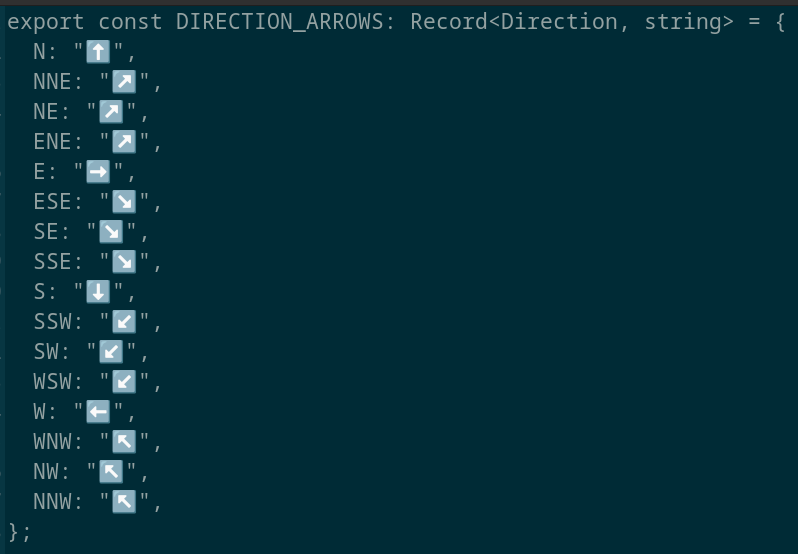
\includegraphics[height = 5cm]{images/directionCode.png}%
            \end{figure}
        \end{column}
    \end{columns}
    
\end{frame}